\esSezione{Sistema PO/PC}\label{sec:esercizio6-1}

\begin{traccia}
Progettare, implementare in VHDL e verificare mediante simulazione un sistema dotato di una memoria ROM di N locazioni da 8 bit ciascuna, una macchina combinatoria M in grado di trasformare (secondo una funzione a scelta dello studente) la stringa di 8 bit letta dalla ROM in una stringa di 4 bit, e una memoria MEM di N locazioni che memorizza la stringa in output da M.

Il sistema si avvia in corrispondenza di un segnale di START che viene fornito esternamente. Una volta avviato, tramite un'apposita unità di controllo che gestisce la tempificazione del sistema, viene scandita una locazione alla volta della ROM e viene scritta la corrispondente locazione di MEM. Gli indirizzi di memoria sono forniti da un contatore. Le memorie ROM e MEM hanno rispettivamente un read e un write sincrono.
\end{traccia}


\progetto

Il sistema si divide in parte operativa e parte di controllo. Il top module \texttt{sistema} istanzia cinque componenti:
\begin{enumerate}
  \item Control Unit (\texttt{control\_unit});
  \item ROM (\texttt{rom});
  \item macchina combinatoria $M$ (\texttt{onecount});
  \item memoria (\texttt{mem});
  \item contatore (\texttt{counter\_mod}).
\end{enumerate}

L'indirizzo, comune a ROM e MEM, è fornito dal contatore. La ROM restituisce il byte letto su \texttt{rom\_data}; la macchina $M$ lo trasforma in \texttt{m\_data}, che è il dato in ingresso alla MEM. L'unità di controllo riceve \texttt{start} e il riporto \texttt{tc} del contatore e produce i comandi \texttt{rd} (lettura della ROM), \texttt{we} (scrittura della MEM), \texttt{cnt\_en} (avanzamento del contatore) e l'uscita \texttt{done}. La funzione scelta per $M$ è il conteggio degli '1' presenti nel byte, così il risultato, compreso tra 0 e 8, sta su 4 bit.

Lo schema a blocchi dell'architettura è riportato in Figura~\ref{fig:esercizio6-1:schema}: in basso la parte operativa, in alto l'unità di controllo con i segnali di controllo e di stato scambiati con essa.

\begin{figure}[H]
  \centering
  \scalebox{0.93}{%
  \begin{tikzpicture}[font=\sffamily\small]
    \node[blocco, minimum width=1.8cm] (cnt) at (0,0) {\texttt{counter\_mod}};
    \node[blocco, minimum width=1.8cm] (rom) at (4,0) {\texttt{rom}};
    \node[blocco, minimum width=1.8cm] (m) at (8,0) {$M$\\[-2pt]\scriptsize\texttt{onecount}};
    \node[blocco, minimum width=1.8cm] (mem) at (12,0) {\texttt{mem}};
    \node[ctrl, minimum width=6.5cm] (cu) at (6,3.2) {\texttt{control\_unit}};

    \draw[bus] (cnt) -- node[pos=0.25, above=3pt, font=\scriptsize]{\texttt{addr}} node[pos=0.55, sloped, inner sep=1pt]{/} node[pos=0.55, below=3pt, font=\scriptsize]{4} (rom);
    \draw[bus] (rom) -- node[pos=0.28, above=3pt, font=\scriptsize]{\texttt{rom\_data}} node[pos=0.75, sloped, inner sep=1pt]{/} node[pos=0.75, below=3pt, font=\scriptsize]{8} (m);
    \draw[bus] (m) -- node[pos=0.28, above=3pt, font=\scriptsize]{\texttt{m\_data}} node[pos=0.75, sloped, inner sep=1pt]{/} node[pos=0.75, below=3pt, font=\scriptsize]{4} (mem);
    \draw[bus] (2.8,0) -- (2.8,-1.2) -- node[below, font=\scriptsize]{\texttt{addr} ($\to$ \texttt{waddr})} (11.6,-1.2) -- (11.6,-0.5);
    \fill (2.8,0) circle (1.5pt);
    \draw[bus,<-] (12.4,-0.5) -- (12.4,-1.2) node[below, font=\scriptsize]{\texttt{raddr}};
    \draw[bus] (mem.east) -- ++(1,0) node[right, font=\scriptsize]{\texttt{dout}};

    \draw[seg] ([xshift=-3cm]cu.south) -- ++(0,-0.6) -| (cnt.north);
    \node[font=\scriptsize, left] at (2.9,2.3) {\texttt{cnt\_en}};
    \draw[seg] ([xshift=-1cm]cu.south) -- ++(0,-0.9) -| (rom.north);
    \node[font=\scriptsize, right] at (5.1,2.1) {\texttt{rd}};
    \draw[seg] ([xshift=3cm]cu.south) -- ++(0,-0.6) -| (mem.north);
    \node[font=\scriptsize, right] at (9.1,2.3) {\texttt{we}};
    \draw[seg] (cnt.west) -- ++(-0.7,0) |- node[pos=0.25, left, font=\scriptsize]{\texttt{tc}} (cu.west);
    \draw[seg,<-] ([xshift=-0.8cm]cu.north) -- ++(0,0.6) node[above, font=\scriptsize]{\texttt{start}};
    \draw[seg,<-] ([xshift=0.8cm]cu.north) -- ++(0,0.6) node[above, font=\scriptsize]{\texttt{rst}};
    \draw[seg] (cu.east) -- ++(1,0) node[right, font=\scriptsize]{\texttt{done}};
  \end{tikzpicture}}
  \caption{Architettura PO/PC del sistema. \texttt{clk} raggiunge tutti i blocchi sincroni e \texttt{rst} anche il contatore; non sono disegnati.}
  \label{fig:esercizio6-1:schema}
\end{figure}

\implementazione

Partiamo dai componenti della parte operativa. La ROM è descritta dall'entità \texttt{rom}, con generic \texttt{N} (locazioni) e \texttt{A} (bit di indirizzo) e porte \texttt{clk}, \texttt{rd}, \texttt{addr} (\texttt{A} bit) e \texttt{data} (8 bit). L'architettura \texttt{behavioral} contiene la costante \texttt{CONTENT}, un array di \texttt{N} byte con sedici valori iniziali e gli altri a \texttt{x"00"}. Un process sensibile a \texttt{clk} carica \texttt{data} sul fronte di salita solo se \texttt{rd} vale '1', quindi la lettura è sincrona. Un \texttt{assert} con severità \texttt{failure} controlla che \texttt{N} sia indirizzabile su \texttt{A} bit. 

\vhdlfile{esercizio6-1/rom.vhd}{Implementazione della ROM}{lst:esercizio6-1:rom}

La macchina combinatoria $M$ è l'entità \texttt{onecount}, con ingresso \texttt{x} a 8 bit e uscita \texttt{y} a 4 bit. Un process sensibile a \texttt{x} azzera una variabile \texttt{n} di tipo \texttt{unsigned} e la incrementa per ogni bit di \texttt{x} pari a '1', con un ciclo \texttt{for} sugli otto indici; \texttt{y} è il risultato convertito in \texttt{std\_logic\_vector}. Senza clock, la rete è puramente combinatoria.

\vhdlfile{esercizio6-1/onecount.vhd}{Implementazione della macchina combinatoria $M$ (conteggio degli '1')}{lst:esercizio6-1:onecount}

L'entità \texttt{mem} ha generic \texttt{N}, \texttt{A} e \texttt{W} (larghezza del dato, 4 per default) e porte \texttt{clk}, \texttt{we}, \texttt{waddr}, \texttt{din}, oltre a \texttt{raddr} e \texttt{dout}, aggiunte per consentire al testbench di leggere il contenuto. La scrittura avviene in un process sincrono, quando \texttt{we} vale '1'; la lettura su \texttt{dout} è invece un assegnamento concorrente, quindi asincrona. Le locazioni sono inizializzate a tutti '1'. La MEM espone quindi anche un'uscita.

\vhdlfile{esercizio6-1/mem.vhd}{Implementazione della memoria MEM}{lst:esercizio6-1:mem}

Il contatore è \texttt{counter\_mod}, già presentato nell'esercizio 5.1 (listato~\ref{lst:esercizio5-1:counter-mod}). Nel sistema è istanziato con \texttt{M} pari a \texttt{N} e \texttt{W} pari a \texttt{A}, con \texttt{load} a '0' e ingresso \texttt{d} a zero; l'uscita \texttt{tc} vale '1' quando il contatore è abilitato e si trova sull'ultimo valore.

L'unità di controllo \texttt{control\_unit} è una FSM di tipo Moore con quattro stati (\texttt{S\_IDLE}, \texttt{S\_READ}, \texttt{S\_WRITE}, \texttt{S\_DONE}), descritta con due process. Il process \texttt{f\_controllo}, sensibile a \texttt{stato\_corrente}, \texttt{start} e \texttt{tc}, assegna dei valori di default alle uscite e calcola lo stato prossimo; il process \texttt{mem\_stato} aggiorna \texttt{stato\_corrente} sul fronte di salita di \texttt{clk}, con reset sincrono verso \texttt{S\_IDLE}. Gli stati si comportano così:
\begin{enumerate}
  \item in \texttt{S\_IDLE} si attende \texttt{start} a '1' per passare in \texttt{S\_READ};
  \item in \texttt{S\_READ} viene attivato \texttt{rd} e si passa in \texttt{S\_WRITE};
  \item in \texttt{S\_WRITE} vengono attivati \texttt{we} e \texttt{cnt\_en}; se \texttt{tc} vale '1' si va in \texttt{S\_DONE}, altrimenti si torna in \texttt{S\_READ};
  \item in \texttt{S\_DONE} viene attivato \texttt{done}, e si torna in \texttt{S\_IDLE} solo quando \texttt{start} torna a '0'.
\end{enumerate}
Ogni locazione richiede quindi due cicli di clock: nel primo la ROM campiona l'indirizzo, nel secondo il dato elaborato da $M$ è disponibile e viene scritto in MEM nello stesso fronte in cui il contatore avanza. 

\vhdlfile{esercizio6-1/control_unit.vhd}{Implementazione della Control Unit}{lst:esercizio6-1:cu}

Il top module \texttt{sistema} ha generic \texttt{N} (16) e \texttt{A} (4) e porte \texttt{clk}, \texttt{rst}, \texttt{start} in ingresso, \texttt{done} in uscita, oltre a \texttt{raddr} e \texttt{dout} per la lettura della MEM. L'architettura \texttt{structural} istanzia i cinque componenti con port mapping e dichiara i segnali interni \texttt{addr}, \texttt{rom\_data}, \texttt{m\_data}, \texttt{rd}, \texttt{we}, \texttt{cnt\_en} e \texttt{tc}.

\vhdlfile{esercizio6-1/sistema.vhd}{Implementazione del top module del sistema}{lst:esercizio6-1:sistema}

\simulazione

Il testbench \texttt{sistema\_tb} ha un'entità senza porte e istanzia il top module come \texttt{dut} con \texttt{N} pari a 16 e \texttt{A} pari a 4. Il clock ha periodo di \SI{10}{ns}, generato da un process dedicato. Il process \texttt{stim} esegue questi passi:
\begin{itemize}
  \item \texttt{rst} a '1' per due periodi, poi a '0' per altri due;
  \item \texttt{start} a '1' e attesa di \texttt{done} a '1';
  \item attesa di tre periodi, poi \texttt{start} a '0' e altri due periodi;
  \item lettura di tutte le locazioni della MEM tramite \texttt{raddr}, con un \texttt{assert} per ciascuna, confrontata con i valori attesi della costante \texttt{EXP}, con severità \texttt{error}.
\end{itemize}
I valori attesi sono il numero di '1' di ciascun byte della ROM: $0, 8, 1, 1, 4, 4, 4, 4, 7, 7, 2, 4, 6, 1, 4, 4$.

\vhdlfile{esercizio6-1/sistema_tb.vhd}{Testbench del sistema}{lst:esercizio6-1:tb}

Il risultato della simulazione è in figura~\ref{fig:esercizio6-1:simulazione}.

\begin{figure}[H]
  \centering
  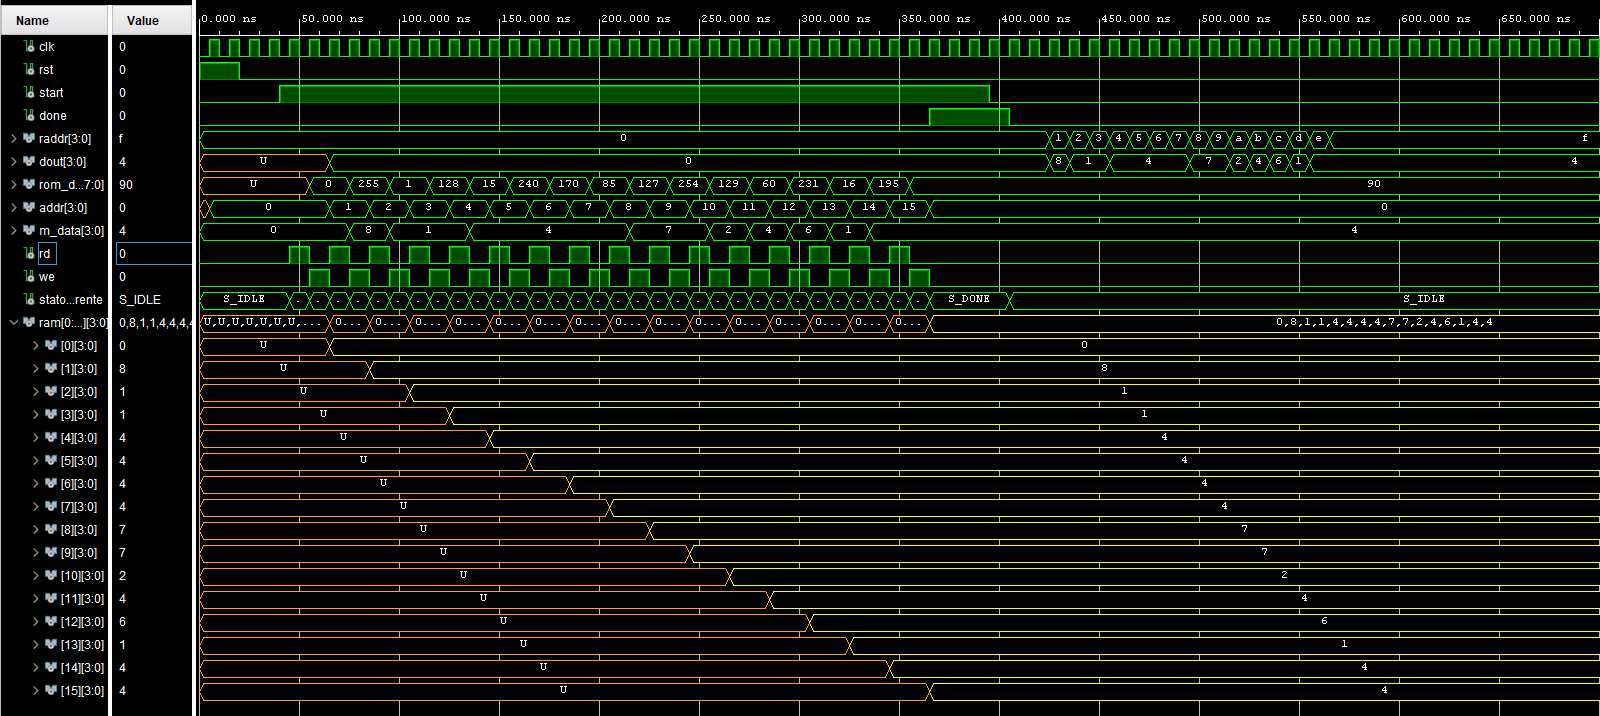
\includegraphics[width=\linewidth]{figure/esercizio6-1/simulazione}
  \caption{Simulazione del sistema PO/PC}
  \label{fig:esercizio6-1:simulazione}
\end{figure}


\begin{risultato}
Il contenuto finale di \texttt{ram} mostrato in figura coincide con i valori attesi di \texttt{EXP}, e \texttt{done} viene attivato una volta al termine della scansione.
\end{risultato}
